\subsection{離散時間 Kalman フィルタを予測と更新から導く}

Kalman フィルタは、モデルに基づく予測と測定値に基づく更新から構成される。この二段構造は、線形確率モデルの条件付き平均と誤差共分散の計算により得られる。LQR の重み行列と区別するため、プロセスノイズの共分散を $Q_{w,k}$、測定ノイズの共分散を $R_{v,k}$ と書く。

離散時間の線形モデルを
\begin{align}
  x_k&=A_{k-1}x_{k-1}+B_{k-1}u_{k-1}+G_{k-1}w_{k-1},\label{eq:kf-state-model}\\
  y_k&=C_kx_k+v_k
  \label{eq:kf-measurement-model}
\end{align}
とする。状態は $x_k\in\R^n$、入力は $u_k\in\R^m$、測定は $y_k\in\R^p$ である。$w_k$ はモデル化できなかった外乱や離散化誤差をまとめたプロセスノイズ、$v_k$ はセンサノイズである。仮定は
\begin{align}
  E[w_i]&=0,
  &E[v_i]&=0,\\
  E[w_iw_j^\T]&=Q_{w,i}\delta_{ij},
  &E[v_iv_j^\T]&=R_{v,i}\delta_{ij},\\
  E[w_iv_j^\T]&=0
\end{align}
であり、初期推定誤差 $x_0-\hat{x}_{0|0}$ もすべての $w_i,v_i$ と相関しないとする。ここで $\delta_{ij}$ は $i=j$ で 1、そうでなければ 0 になるクロネッカーのデルタである。さらに予測平均の式では、$w_{k-1}$ が過去の測定履歴 $\mathcal{Y}_{k-1}$ に対してゼロ条件付き平均
\begin{equation}
  E[w_{k-1}\mid\mathcal{Y}_{k-1}]=0
\end{equation}
を持つことを仮定する。独立な白色ノイズを仮定すれば、この条件は満たされる。条件付き平均推定として最適性を述べるときは、これらの確率変数が同時正規分布に従う線形ガウス系を仮定する。ガウス性を仮定しない場合、以下の更新は線形な革新更新に制限した最小平均二乗誤差推定として解釈する。

時刻 $k$ までの測定履歴を
\begin{equation}
  \mathcal{Y}_k=\{y_0,y_1,\ldots,y_k\}
\end{equation}
と書く。推定値 $\hat{x}_{k|k}$ は $\mathcal{Y}_k$ を見た後の状態推定、$\hat{x}_{k|k-1}$ は $\mathcal{Y}_{k-1}$ までを見て時刻 $k$ を予測した値である。対応する推定誤差と共分散を
\begin{align}
  e_{k|k}&=x_k-\hat{x}_{k|k},
  &P_{k|k}&=E[e_{k|k}e_{k|k}^\T\mid\mathcal{Y}_k],\\
  e_{k|k-1}&=x_k-\hat{x}_{k|k-1},
  &P_{k|k-1}&=E[e_{k|k-1}e_{k|k-1}^\T\mid\mathcal{Y}_{k-1}]
\end{align}
と定義する。

まず予測を導く。$u_{k-1}$ は時刻 $k-1$ で与えた既知の入力なので、\weq{kf-state-model} の条件付き期待値を取ると
\begin{align}
  \hat{x}_{k|k-1}
  &=E[x_k\mid\mathcal{Y}_{k-1}]\\
  &=A_{k-1}E[x_{k-1}\mid\mathcal{Y}_{k-1}]+B_{k-1}u_{k-1}
    +G_{k-1}E[w_{k-1}\mid\mathcal{Y}_{k-1}]\\
  &=A_{k-1}\hat{x}_{k-1|k-1}+B_{k-1}u_{k-1}
\end{align}
となる。最後の等号では、$E[w_{k-1}\mid\mathcal{Y}_{k-1}]=0$ を使った。予測誤差は
\begin{align}
  e_{k|k-1}
  &=x_k-\hat{x}_{k|k-1}\\
  &=A_{k-1}(x_{k-1}-\hat{x}_{k-1|k-1})+G_{k-1}w_{k-1}\\
  &=A_{k-1}e_{k-1|k-1}+G_{k-1}w_{k-1}
\end{align}
である。したがって共分散は
\begin{align}
  P_{k|k-1}
  &=E[e_{k|k-1}e_{k|k-1}^\T\mid\mathcal{Y}_{k-1}]\\
  &=A_{k-1}P_{k-1|k-1}A_{k-1}^\T+G_{k-1}Q_{w,k-1}G_{k-1}^\T
\end{align}
になる。途中に出る $E[e_{k-1|k-1}w_{k-1}^\T]$ とその転置は、推定誤差と新しいプロセスノイズが無相関であるため消える。

次に測定値に基づく更新を導く。予測された測定値は
\begin{equation}
  \hat{y}_{k|k-1}=C_k\hat{x}_{k|k-1}
\end{equation}
であり、実際の測定との差
\begin{equation}
  \nu_k=y_k-\hat{y}_{k|k-1}=y_k-C_k\hat{x}_{k|k-1}
\end{equation}
を革新という。\weq{kf-measurement-model} を代入すると
\begin{align}
  \nu_k
  &=C_kx_k+v_k-C_k\hat{x}_{k|k-1}\\
  &=C_ke_{k|k-1}+v_k
\end{align}
なので、その共分散は
\begin{align}
  S_k
  &=E[\nu_k\nu_k^\T\mid\mathcal{Y}_{k-1}]\\
  &=C_kP_{k|k-1}C_k^\T+R_{v,k}
\end{align}
である。$S_k$ は革新共分散と呼ばれ、予測誤差共分散を測定空間へ写した項と測定ノイズ共分散の和である。

更新式を、革新に行列ゲイン $K_k$ を掛けて足す形
\begin{equation}
  \hat{x}_{k|k}=\hat{x}_{k|k-1}+K_k\nu_k
  \label{eq:kf-update-mean}
\end{equation}
に限って考える。以下では、線形な革新更新の範囲で $K_k$ を選ぶ。更新後の誤差は
\begin{align}
  e_{k|k}
  &=x_k-\hat{x}_{k|k}\\
  &=x_k-\hat{x}_{k|k-1}-K_k(C_ke_{k|k-1}+v_k)\\
  &=(I-K_kC_k)e_{k|k-1}-K_kv_k.
\end{align}
したがって、任意の $K_k$ に対する更新後共分散は次式で表される。線形ガウス仮定のもとでは、この共分散は革新の実現値に依存しない。ガウス性を仮定しない場合、次式は $\mathcal{Y}_{k-1}$ で条件付けた線形最小平均二乗誤差の共分散として解釈する。
\begin{equation}
  P_{k|k}(K_k)
  =(I-K_kC_k)P_{k|k-1}(I-K_kC_k)^\T+K_kR_{v,k}K_k^\T
  \label{eq:joseph-form-general}
\end{equation}
である。この式でも、$e_{k|k-1}$ と $v_k$ の交差共分散が 0 であることを使っている。

ゲインは $\tr P_{k|k}(K_k)$ を最小にするように選ぶ。記号を軽くするため、この段落だけ
\begin{equation}
  P^-=P_{k|k-1},
  \qquad C=C_k,
  \qquad R=R_{v,k},
  \qquad S=CP^-C^\T+R
\end{equation}
と書く。\weq{joseph-form-general} を展開すると
\begin{align}
  P(K)
  &=P^- -KCP^- -P^-C^\T K^\T+K(CP^-C^\T+R)K^\T\\
  &=P^- -KCP^- -P^-C^\T K^\T+KSK^\T.
\end{align}
ここで
\begin{equation}
  K_\text{opt}=P^-C^\T S^{-1}
\end{equation}
と置けば、$K_\text{opt}S=P^-C^\T$ が成り立つ。平方完成と同じ形に整理すると
\begin{align}
  P(K)
  &=P^- -K_\text{opt}S K_\text{opt}^\T
    +(K-K_\text{opt})S(K-K_\text{opt})^\T.
\end{align}
$R=R^\T>0$ なら $S>0$ であり、最後の項は半正定値である。したがって $\tr P(K)$ を最小にするのは $K=K_\text{opt}$ で、Kalman ゲインは
\begin{equation}
  K_k=P_{k|k-1}C_k^\T
  (C_kP_{k|k-1}C_k^\T+R_{v,k})^{-1}
  \label{eq:kf-gain-derived}
\end{equation}
となる。

最適ゲインを代入した共分散更新は、簡略形として
\begin{align}
  P_{k|k}
  &=P_{k|k-1}-K_kS_kK_k^\T\\
  &=(I-K_kC_k)P_{k|k-1}
  \label{eq:kf-covariance-simple}
\end{align}
と書ける。二つ目の等号では $K_kS_k=P_{k|k-1}C_k^\T$ を使った。数式上はこれでよいが、有限精度演算では丸め誤差によって $P_{k|k}$ の対称性や半正定値性が崩れることがある。そのため実装では、代数的には同値な Joseph 形式
\begin{equation}
  P_{k|k}
  =(I-K_kC_k)P_{k|k-1}(I-K_kC_k)^\T+K_kR_{v,k}K_k^\T
  \label{eq:kf-joseph-form}
\end{equation}
を用いる。Joseph 形式は左右対称な積で構成されるため、共分散行列の対称性および半正定値性を保ちやすい。

以上をまとめると、離散時間 Kalman フィルタは
\begin{align}
  \hat{x}_{k|k-1}&=A_{k-1}\hat{x}_{k-1|k-1}+B_{k-1}u_{k-1},\\
  P_{k|k-1}&=A_{k-1}P_{k-1|k-1}A_{k-1}^\T
    +G_{k-1}Q_{w,k-1}G_{k-1}^\T,\\
  \nu_k&=y_k-C_k\hat{x}_{k|k-1},\\
  S_k&=C_kP_{k|k-1}C_k^\T+R_{v,k},\\
  K_k&=P_{k|k-1}C_k^\T S_k^{-1},\\
  \hat{x}_{k|k}&=\hat{x}_{k|k-1}+K_k\nu_k,\\
  P_{k|k}&=(I-K_kC_k)P_{k|k-1}(I-K_kC_k)^\T+K_kR_{v,k}K_k^\T
\end{align}
で与えられる。$G_{k-1}=I$ とすれば、$P_{k|k-1}=AP_{k-1|k-1}A^\T+Q$ の形に一致する。

一次元で $C=1$ とすれば、革新共分散は $S=P^-+R$、ゲインは
\begin{equation}
  K=\frac{P^-}{P^-+R}
\end{equation}
である。予測分散 $P^-$ が大きいほど測定値の重みが大きくなり、測定ノイズ分散 $R$ が大きいほど予測値の重みが大きくなる。たとえば熱系の室温推定では、外乱や未モデル化熱流が大きい場合に $Q_w$ を大きく設定し、温度センサの分散が大きい場合に $R_v$ を大きく設定する。

\subsubsection{LQR 重みと Kalman 共分散の可視化}

二次形式の重みは、式だけで扱うと単なる係数として残りやすい。しかし閉ループ応答、入力指令、リカッチ方程式の収束、推定誤差共分散を同じモデルで並べると、重みが設計上のどの妥協に対応するかを確認できる。図\ref{fig:lqr-kalman-examples}では、サンプル周期 $h=0.1\,\mathrm{s}$ の二重積分器
\begin{equation}
  x_{k+1}
  =
  \begin{bmatrix}
    1 & h\\
    0 & 1
  \end{bmatrix}x_k
  +
  \begin{bmatrix}
    h^2/2\\
    h
  \end{bmatrix}u_k,
  \qquad
  y_k=\begin{bmatrix}1&0\end{bmatrix}x_k+v_k
\end{equation}
を用いている。状態は位置偏差と速度偏差であり、測定は位置だけである。上段左は $Q_x=\diag(1,0.08)$ を固定して入力重み $R_u$ を変えたときの位置偏差、上段右は対応する LQR の入力指令 $u_c=-Kx$ である。$R_u$ が小さいほど偏差は早く消えるが、入力指令は大きくなり、図中の点線で示した入力限界を越えやすくなる。ここで描いているのは制御器が要求する指令 $u_c$ であり、実際のアクチュエータに飽和があれば対象へ入る入力は $u_a=\operatorname{sat}(u_c)$ である。したがって実装検証では、推定器とシミュレーションに $u_c$ ではなく実際に印加された $u_a$ を渡す必要がある。

\begin{figure}[tb]
\centering
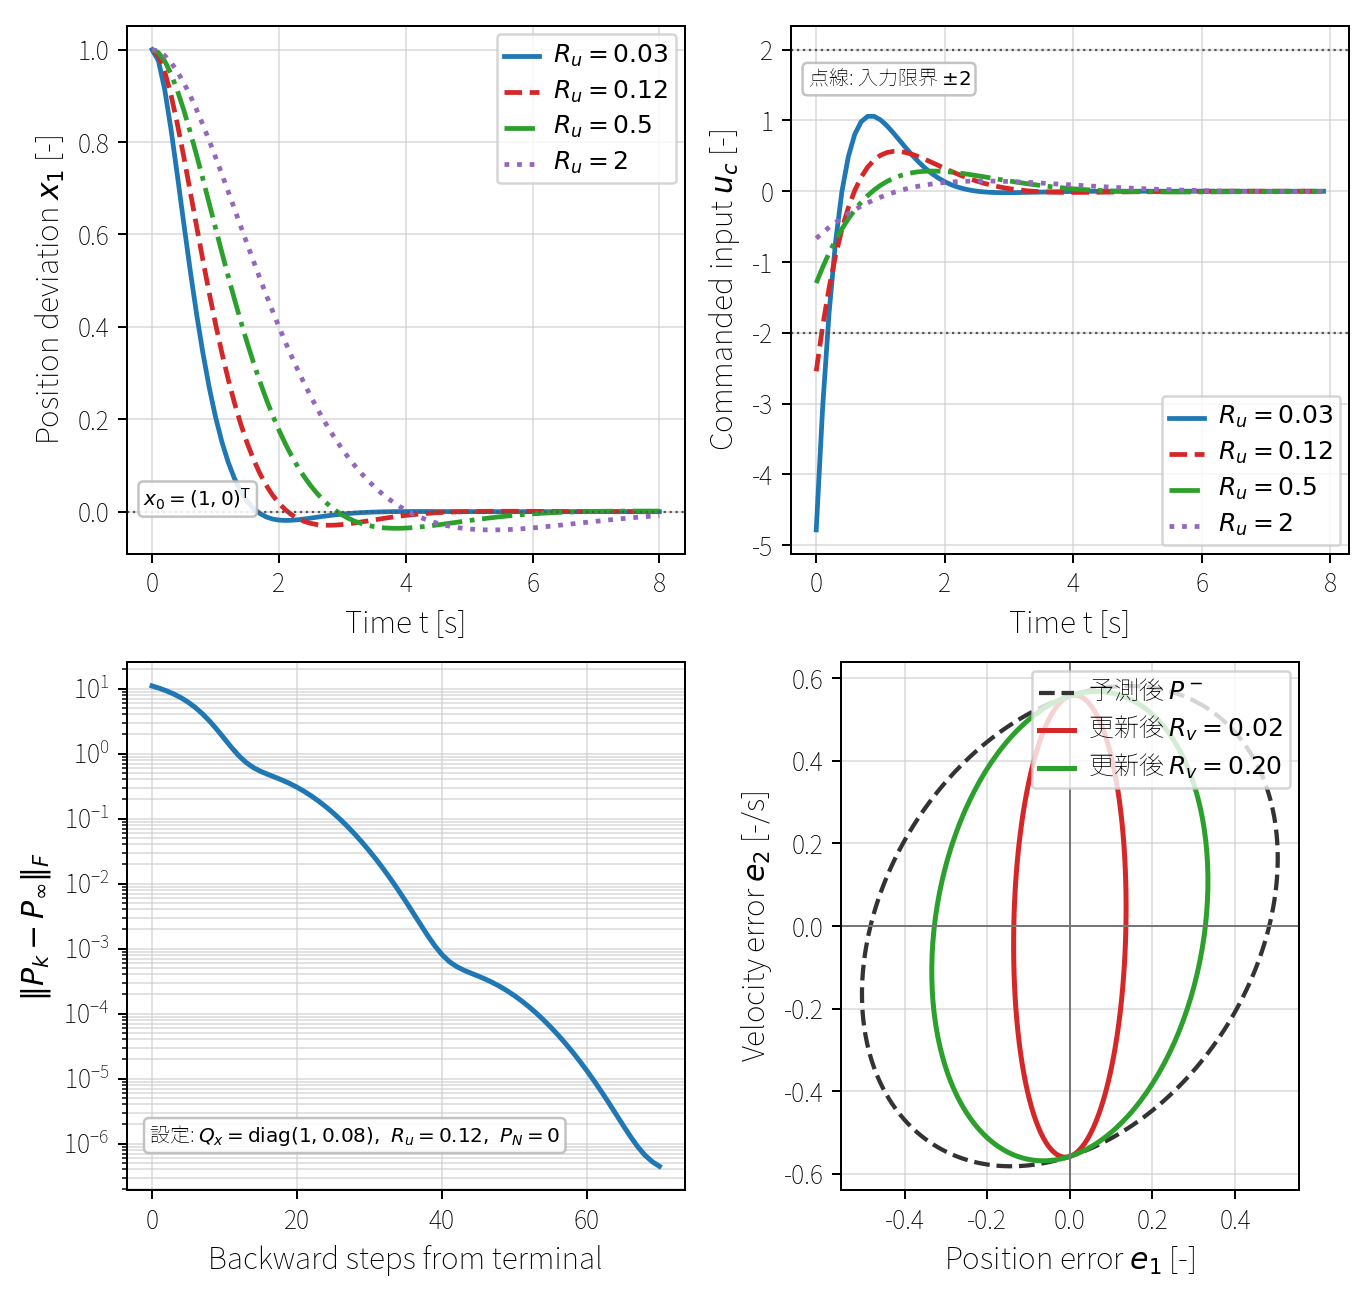
\includegraphics[width=0.95\linewidth,bb=0 0 1368 1296]{figures/lqr_kalman_examples.png}
\caption{二重積分器に対する LQR と Kalman フィルタの調整例。上段は入力重み $R_u$ による状態応答と入力指令の変化であり、入力限界を点線で示している。左下は有限ホライズンの後退リカッチ再帰が定常解へ近づく様子である。右下は予測後の誤差共分散楕円が位置測定によって更新される様子であり、測定ノイズ分散 $R_v$ が小さいほど測定方向の不確かさが強く縮む。}
\label{fig:lqr-kalman-examples}
\end{figure}

左下のリカッチ再帰では、終端条件から後ろ向きに計算した $P_k$ が定常解 $P_\infty$ に近づく。これはホライズンを長くしたとき、現在時刻から十分遠い終端条件の影響が薄れ、無限ホライズン LQR のゲインへ近づくことを表す。右下の共分散楕円は、予測で広がった不確かさが測定更新で縮む過程を示す。位置だけを測っているので、主に位置方向の幅が縮み、速度方向は状態方程式との相関を通じて間接的に修正される。$R_v$ を大きくすると測定を疑うため、更新後楕円は予測楕円に近く残る。

\begin{practice}[重みと共分散図の確認]
図\ref{fig:lqr-kalman-examples}を用いて、$R_u=0.03$ と $R_u=2$ の応答を比較せよ。整定の速さ、最大入力指令、入力限界を越える有無を評価し、実際の入力が飽和する場合に LQR の線形設計と閉ループシミュレーションの結果がずれる理由を説明せよ。さらに右下の共分散楕円について、$R_v$ を大きくしたとき Kalman ゲインが小さくなることを、楕円の縮み方と $K=P^-C^\T(CP^-C^\T+R_v)^{-1}$ から確認せよ。
\end{practice}
